\documentclass[a0,final]{a0poster}
%%%Load packages
\usepackage{multicol} 			%3-column layout
\usepackage[left=2cm,right=2cm,bottom=0cm,top=0cm]{geometry}			%Reset margins
\usepackage{mathpazo}			%Load palatino font & pazo math
\usepackage{color}				%Needed for colour boxes & coloured text


\usepackage{graphicx}     		%Needed to import images

\usepackage[]{algorithm2e}



\DeclareGraphicsExtensions{.pdf,.png,.jpg}

\graphicspath{ {./images/} }




%%%Define colours and lengths
\definecolor{headingcol}{rgb}{1,1,1}			%Colour of main title
\definecolor{boxcol}{rgb}{0.7,0.2,0.2}		%Edge-colour of box and top banner
\fboxsep=1cm							%Padding between box and text
\setlength{\columnsep}{2cm}				%Set spacing between columns

%%%Format title
\makeatletter							%Needed to include code in main file
\renewcommand\@maketitle{%
\null									%Sets position marker
{
\color{headingcol}\sffamily\VERYHuge		%Set title font and colour
\@title \par}%
\vskip 0.6em%
{
\color{white}\sffamily\large				%Set author font and colour
\lineskip .5em%
\begin{tabular}[t]{l}%
\@author
\end{tabular}\par}%
\vskip 1cm
\par
}
\makeatother

\title{BA Scale Free Networks}

\author{Dalwinder Bagdi, Tanvi Bhardwaj, Ankeet Dhanji, Dani Grayston, Alexandru Stoenescu \& Shuai Wang (Robert)\\
University of Manchester - Group 5}

\begin{document}

\hspace{-3cm}								%Align with edge of page, not margin
\colorbox{boxcol}{							%Coloured banner across top
\begin{minipage}{1189mm}					%Minipage for title contents
\maketitle
\end{minipage}}
\vspace{1cm}

\begin{multicols}{3}							%Use 3-column layout
\raggedcolumns							%Don't stretch contents vertically

%%%Column1
\section{Introduction}
Lorem ipsum dolor sit amet, consectetuer adipiscing elit. Ut dui. Vivamus ullamcorper. Pellentesque metus dui, facilisis nec, aliquet ut, ultrices quis, ipsum. Mauris semper venenatis nunc. Nunc et leo. Morbi quis tortor quis ipsum rhoncus faucibus. Praesent nunc. Aliquam justo. Nullam vitae leo. Nam imperdiet scelerisque orci.\\
\\
Donec quis urna. Vestibulum ante ipsum primis in faucibus orci luctus et ultrices posuere cubilia Curae; Integer vel ante a tortor sollicitudin elementum. Duis tortor est, tincidunt non, dapibus sed, tincidunt in, elit. Sed auctor. Sed libero augue, sollicitudin ut, vehicula quis, feugiat feugiat, risus. Phasellus lobortis. Cras ut tellus sit amet neque porta convallis. Quisque ut mi. Cras elit nunc, ultrices in, tempus sit amet, semper in, purus.\\
\\
Vivamus interdum erat non massa. Nullam condimentum metus sed dui. Nam gravida risus eu dui. Donec quis risus sit amet elit semper imperdiet. Aliquam ut pede nec orci pharetra ultrices. Integer sed velit quis tellus sollicitudin commodo. Phasellus scelerisque tellus ut justo. Vivamus condimentum leo quis lectus. Aliquam sem massa, tincidunt ac, venenatis at, pulvinar vulputate, lectus. Nulla sit amet libero. Nullam fermentum nunc et sapien luctus lobortis. Aenean lectus purus, porta at, tincidunt in, aliquam vel, nisi. Cum sociis natoque penatibus et magnis dis parturient montes, nascetur ridiculus mus. Vestibulum quis velit. Nam tincidunt nisi sed erat. Sed vel enim eu lectus mattis convallis. In vulputate tincidunt erat. Ut nec ligula id tellus aliquam aliquam. In lectus erat, malesuada sed, dignissim a, gravida sit amet, justo. Donec nulla.


\section{Analysis}
\subsection{Parameters}
There are three parameters in this algorithm. They are the totoal number of nodes T;  Initial number of nodes $n_0$ and the minimum degree M. \\
\begin{description} 
  \item[Initial number of nodes $n_0$] should be a small number. It is the number of nodes a graph start with.
  \item[Total number of nodes to be added T] is the total timestep. Increasing T will add more nodes to the network, making it more dense. The nodes that have a high degree will continue to grow rapidly (in terms of links) and the nodes with less degree will not gain as many links.
  \item[Minimum degree M] is the minimum number of links the new node starts with. It will be linked M times to existing nodes according to their probability of being linked. If M is large then the new node is more likely to gain extra connections in subsequent iterations of the algorithm, otherwise not.
\end{description}

\columnbreak

%%%Column 2
\section*{Algorithms}


\begin{algorithm}[H]
 \KwData{Total number of nodes to be added T; \\
       Initial number of nodes $n_0$; \\
       Minimum degree M.\\}
 \KwResult{scale-free multigraph G}
Add $n_0$ nodes to G.\\
%Connect every node in G to every other node in G, i.e. create a complete graph. \\
t = 0
 \While{!t$<$T}{
    Create a new node i.\\

 \While{!m$<$M}{
Pick a node j at random from the graph G with probability of each node as P[j].\\
Pick a real number R uniformly at random between 0 and 1.\\
     \If{P[j] $>$ R}{
        add j to i's adjacency list\\
 	m++
    }
Add i to the adjacency list of each node in its adjacency list.\\
Add i to to the graph.\\
}
$ P[i] = \frac{k_i}{\sum\limits_{k=1}^N} k_j$, N = $n_0$ + t -1\\
t++
    }
return graph G\\
 \caption{BA Network Generation Algorithm}
\end{algorithm}


\columnbreak

%%%Column 3
\section*{Examples of Scale Free Networks}

There are many various examples of Scale Free Networks. These range from Air Traffic Networks to the Internet. Below is an example of a Scale Free network that was generated by the BA algorithm.
\newline
{\centering
\centerline{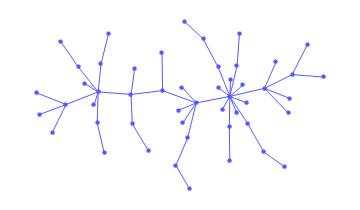
\includegraphics[scale=1.5]{BA.jpg}}}
\newline
The BA network above is created using 50 nodes that each initially had a degree of 1.
After applying the BA algorithm, it is visible there are very few nodes with a high degree. This is due to nodes that have a higher degree have a high probability of gaining more links, thus the "rich" are becoming "richer". This also means that the new network created follows Power Law distribution.
\newline

\centerline{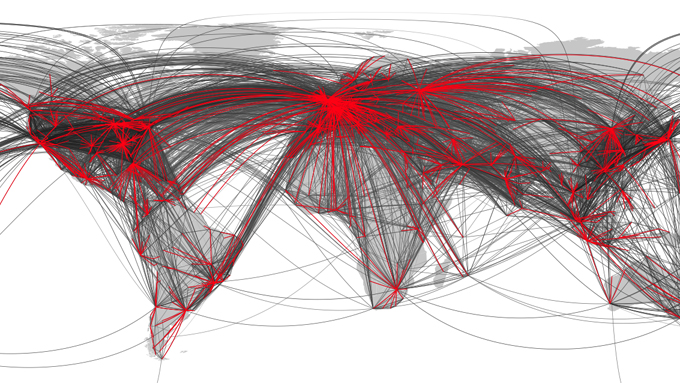
\includegraphics{airtraffic.jpg}}

The figure above shows the Global Air Traffic Network. It shows the there are a few internation airports (nodes) in the world that connect (link) to many different places. However most airports only connect to a small number of places, thus these airports have a small degree. Again this Air Traffic Network has the Power Law Distribution property.

\section*{Conclusion}
In this poster, a Scale Free BA network was defined, An algorithm was presented. Several parameters were introduced. The results were analysed as these parameters vary. There is XX difference when increasing the size of the network and similarities were investigated and compared with small real-world networks. In addition, topological properties were analysed. 
%\nocite*

\bibliographystyle{plain}
\bibliography{halobib}

\end{multicols}
\end{document}
